\chapter{Planificacion}
\section{Introducción}
En este capítulo vamos a realizar la planificación para el desarrollo del proyecto, la cual va a servir para poder
realizar un control de los avances del producto y asegurar que se cumplan los objetivos marcados en cada sprint (o iteración).
Para ello, se utilizarán algunos elementos de la metodología SCRUM, como son los sprints, las historias de usuario y el product backlog, etc. Es importante esto último
porque solo usaremos algunos principios y conceptos de metodologías ágiles pero no vamos a seguir al pie de la letra ninguna de ellas debido
a las condiciones en las que se va a desarrollar el proyecto (no hay un cliente real, no hay un equipo de desarrollo real, etc.).

\section{Velocidad}
A continuación vamos a estimar la velocidad inicial de trabajo que se tendrá en el desarrollo. Esta será una aproximación que nos ayudará a estimar la cantidad de trabajo que se debería realizar
en cada iteración. Sin embargo, esta podrá variar y ajustarse a lo largo del proyecto en función de la cantidad de trabajo que se logre completar en cada sprint.

Para calcular la velocidad, vamos a considerar las horas de trabajo que se pretenden dedicar al proyecto cada día y tratar de estimar cuanta cantidad de trabajo se podría realizar.

\begin{itemize}
\item Podríamos decir que partimos de un "equipo de desarrollo" de 1 miembro.
\item Se pretende dedicar 5 horas al día de trabajo aproximadamente.
\item Cada Sprint dura 2 semanas (14 días). Si cada día trabajamos 5 horas aproximadamente, obtenemos un total de 70 horas en cada Sprint, que equivalen a 3 días de trabajo reales.
\item En mi entorno, se estima que 1 PH es un día de trabajo ideal. Esto quiere decir que en cada jornada de trabajo real, se debería completar 1 PH. Sin embargo, en la realidad, esto no siempre es así ya que es una aproximación.
\item Si multiplicamos un programador por los 3 días de trabajo reales, obtenemos que deberíamos completar \textbf{3 PH} por sprint aproximadamente.
\end{itemize}

\textit{Nota: La duración de los Sprints puede variar en función de factores externos al proyecto. Pero se tratará de que duren 2 semanas para seguir un ritmo de trabajo constante.}

\textit{Nota 2: Puesto que estamos realizando estimaciones y suposiciones para la planificación, esta está sujeta a cambios a lo largo del proyecto.}
\section{Product Backlog}
A continuación, se listarán todas las historias de usuario ordenadas por prioridad de acuerdo a la importancia que tienen para el usuario final del producto.
\begin{itemize}
    \item \textbf{HU1 - } Como usuario quiero registrarme en la aplicación para poder comenzar a utilizar sus funcionalidades. (Prioridad: Alta | Puntos de Historia: 1)
    \item \textbf{HU2 - } Como usuario quiero iniciar sesión en la aplicación para poder acceder a sus funcionalidades. (Prioridad: Alta | Puntos de Historia: 1)
    \item \textbf{HU6 - } Como usuario quiero seleccionar una lección para leer el temario. (Prioridad: Alta | Puntos de Historia: 0.5)
    \item \textbf{HU7 - } Como usuario quiero empezar un test de una lección. (Prioridad: Alta | Puntos de Historia: 0.5)
    \item \textbf{HU26 - } Como usuario quiero responder una pregunta de un test del tipo escritura de texto. (Prioridad: Alta | Puntos de Historia: 0.5)
    \item \textbf{HU8 - } Como usuario quiero responder una pregunta de un test del tipo selección múltiple. (Prioridad: Alta | Puntos de Historia: 0.5)
    \item \textbf{HU9 - } Como usuario quiero responder una pregunta de un test del tipo selección única. (Prioridad: Alta | Puntos de Historia: 0.5)
    \item \textbf{HU10 - } Como usuario quiero responder una pregunta de un test del tipo respuesta por micrófono. (Prioridad: Alta | Puntos de Historia: 3)
    \item \textbf{HU29 - } Como profesor quiero ver una lista de todas las preguntas. (Prioridad: Alta | Puntos de Historia: 0.25)
    \item \textbf{HU11 - } Como usuario quiero ver el resultado de un test. (Prioridad: Media | Puntos de Historia: 0.5)
    \item \textbf{HU13 - } Como usuario quiero ver mi progreso en las lecciones. (Prioridad: Media | Puntos de Historia: 0.5)
    \item \textbf{HU28 - } Como profesor quiero ver una lista de todas las lecciones. (Prioridad: Media | Puntos de Historia: 0.25)
    \item \textbf{HU14 - } Como profesor quiero crear una lección. (Prioridad: Media | Puntos de Historia: 0.5)
    \item \textbf{HU15 - } Como profesor quiero modificar el texto de una lección. (Prioridad: Media | Puntos de Historia: 0.5)
    \item \textbf{HU16 - } Como profesor quiero añadir contenido multimedia a una lección. (Prioridad: Media | Puntos de Historia: 1)
    \item \textbf{HU17 - } Como profesor quiero eliminar contenido multimedia de una lección. (Prioridad: Media | Puntos de Historia: 0.5)
    \item \textbf{HU27 - } Como profesor quiero añadir preguntas a un test del tipo escritura de texto. (Prioridad: Media | Puntos de Historia: 0.5)
    \item \textbf{HU18 - } Como profesor quiero añadir preguntas a un test del tipo selección múltiple. (Prioridad: Media | Puntos de Historia: 0.5)
    \item \textbf{HU19 - } Como profesor quiero añadir preguntas a un test del tipo selección única. (Prioridad: Media | Puntos de Historia: 0.5)
    \item \textbf{HU20 - } Como profesor quiero añadir preguntas a un test del tipo respuesta por micrófono. (Prioridad: Media | Puntos de Historia: 1)
    \item \textbf{HU21 - } Como profesor quiero eliminar preguntas de un test. (Prioridad: Media | Puntos de Historia: 0.25)
    \item \textbf{HU22 - } Como profesor quiero modificar preguntas de un test. (Prioridad: Media | Puntos de Historia: 0.5)
    \item \textbf{HU30 - } Como administrador quiero ver una lista de todos los usuarios. (Prioridad: Media | Puntos de Historia: 0.25)
    \item \textbf{HU24 - } Como administrador quiero modificar los datos de un usuario. (Prioridad: Media | Puntos de Historia: 1)
    \item \textbf{HU25 - } Como administrador quiero eliminar un usuario. (Prioridad: Media | Puntos de Historia: 0.5)
    \item \textbf{HU23 - } Como administrador quiero crear un usuario. (Prioridad: Baja | Puntos de Historia: 1)
    \item \textbf{HU12 - } Como usuario quiero ver el ranking de usuarios. (Prioridad: Baja | Puntos de Historia: 0.5)
    \item \textbf{HU5 - } Como usuario quiero ver el perfil de otros usuarios.  (Prioridad: Baja | Puntos de Historia: 0.5)
    \item \textbf{HU3 - } Como usuario quiero ver los datos personales y los logros de mi perfil. (Prioridad: Media | Puntos de Historia: 0.5)
    \item \textbf{HU4 - } Como usuario quiero editar los datos de mi perfil. (Prioridad: Media | Puntos de Historia: 1)
\end{itemize}

\section{Sprints}
Nuestro proyecto se va a desarrollar en distintos Sprints, que son iteraciones de trabajo que se van a realizar en el proyecto.
Cada Sprint tendrá una duración de 2 semanas, y se pretenden realizar
\subsection{Sprint \#1 - Documentación inicial}
\textit{24/11/2022   -   08/12/2022}

En este Sprint se realizará:
\begin{itemize}

    \item Definición del proyecto y del alcance.
    \item Redactar Capítulo 1 - Introducción.
    \item Redactar Capítulo 2 - Estado del Arte.
\end{itemize}
\subsection{Sprint \#2 - Documentación de requisitos}
En este Sprint se planea realizar:
\textit{08/12/2022   -   12/01/2023}
\begin{itemize}
    \item Revisión de la documentación inicial y corrección de errores.
    \item Redactar Capítulo 3 - Especificación de Requisitos.
\end{itemize}

\subsection{Sprint \#3 - Documentación de HU}
\textit{12/01/2023   -   03/02/2023}
En este Sprint se realizará:
\begin{itemize}
    \item Revisión de la documentación de requisitos y corrección de errores.
    \item Redactar Capítulo 4 - Planificación.
    \item Redactar Capítulo 5 - Análisis del problema.
\end{itemize}
\subsection{Sprint \#4 - Diseño y comienzo del desarrollo}
\textit{03/02/2023   -   17/02/2023}
En este Sprint se terminará la documentación y comenzará el desarrollo con:
\begin{itemize}
    \item Redactar Capítulo 6 - Diseño.
    \item Preparación del backend para el desarrollo.
    \begin{itemize}
        \item Creación de la base de datos.
        \item Creación de los modelos, rutas y controladores del servidor con NodeJS.
    \end{itemize}
    \item Preparación del frontend para el desarrollo (creación de la aplicación de Flutter).
\end{itemize}
\subsection{Sprint \#5 - Registro y login de usuarios}
\textit{17/02/2023   -   03/03/2023}
\begin{itemize}
    \item Realizar la HU1 - Como alumno quiero registrarme en la aplicación. (Prioridad: Alta | Puntos de Historia: 1)
    \item Realizar la HU2 - Como alumno quiero iniciar sesión en la aplicación. (Prioridad: Alta | Puntos de Historia: 1)
    \item Realizar la HU6 - Como usuario quiero seleccionar una lección para leer el temario. (Prioridad: Alta | Puntos de Historia: 0.5)
    \item Realizar la HU7 - Como usuario quiero empezar un test de una lección. (Prioridad: Alta | Puntos de Historia: 0.5)
    \item Realizar la HU29 - Como profesor quiero ver una lista de todas las preguntas. (Prioridad: Alta | Puntos de Historia: 0.25)

\end{itemize}


\subsection{Sprint \#6 - Tests y progreso}
\textit{03/03/2023   -   17/03/2023}
\begin{itemize}
    \item Realizar la HU26 - Como usuario quiero responder una pregunta de un test del tipo escritura de texto. (Prioridad: Alta | Puntos de Historia: 0.5)
    \item Realizar la HU8 - Como usuario quiero responder una pregunta de un test del tipo selección múltiple. (Prioridad: Alta | Puntos de Historia: 0.5)
    \item Realizar la HU9 - Como usuario quiero responder una pregunta de un test del tipo selección única. (Prioridad: Alta | Puntos de Historia: 0.5)
    \item Realizar la HU11 - Como usuario quiero ver el resultado de un test. (Prioridad: Media | Puntos de Historia: 0.5)
    \item Realizar la HU12 - Como usuario quiero ver mi progreso en las lecciones. (Prioridad: Media | Puntos de Historia: 0.5)

\end{itemize}

\subsection{Sprint \#7 - Entrada de micrófono y detección de tono}
\textit{17/03/2023   -   31/03/2023}
\begin{itemize}
    \item Realizar la HU10 - Como usuario quiero responder una pregunta de un test del tipo respuesta por micrófono. (Prioridad: Alta | Puntos de Historia: 3)
\end{itemize}

\subsection{Sprint \#8 - Funcionalidades del profesor con lecciones}
\textit{31/03/2023   -   14/04/2023}
\begin{itemize}

\item Realizar la HU13 - Como usuario quiero ver mi progreso en las lecciones. (Prioridad: Media | Puntos de Historia: 0.5)
\item Realizar la HU28 - Como profesor quiero ver una lista de todas las lecciones. (Prioridad: Media | Puntos de Historia: 0.25)
\item Realizar la HU14 - Como profesor quiero crear una lección. (Prioridad: Media | Puntos de Historia: 0.5)
\item Realizar la HU15 - Como profesor quiero modificar el texto de una lección. (Prioridad: Media | Puntos de Historia: 0.5)
\item Realizar la HU16 - Como profesor quiero añadir contenido multimedia a una lección. (Prioridad: Media | Puntos de Historia: 1)
\item Realizar la HU17 - Como profesor quiero eliminar contenido multimedia de una lección. (Prioridad: Media | Puntos de Historia: 0.5)
\end{itemize}

\subsection{Sprint \#9 - Funcionalidades del profesor con tests}
\textit{14/04/2023   -   28/04/2023}
\begin{itemize}
\item Realizar la HU27 - Como profesor quiero añadir preguntas a un test del tipo escritura de texto. (Prioridad: Media | Puntos de Historia: 0.5)
\item Realizar la HU18 - Como profesor quiero añadir preguntas a un test del tipo selección múltiple. (Prioridad: Media | Puntos de Historia: 0.5)
\item Realizar la HU19 - Como profesor quiero añadir preguntas a un test del tipo selección única. (Prioridad: Media | Puntos de Historia: 0.5)
\item Realizar la HU20 - Como profesor quiero añadir preguntas a un test del tipo respuesta por micrófono. (Prioridad: Media | Puntos de Historia: 1)
\item Realizar la HU21 - Como profesor quiero eliminar preguntas de un test. (Prioridad: Media | Puntos de Historia: 0.25)
\item Realizar la HU22 - Como profesor quiero modificar preguntas de un test. (Prioridad: Media | Puntos de Historia: 0.5)
\end{itemize}

\subsection{Sprint \#10 - Funcionalidades del administrador y ranking}
\textit{28/04/2023   -   12/05/2023}
\begin{itemize}
\item Realizar la HU24 - Como administrador quiero modificar los datos de un usuario. (Prioridad: Media | Puntos de Historia: 1)
\item Realizar la HU30 - Como administrador quiero ver una lista de todos los usuarios. (Prioridad: Media | Puntos de Historia: 0.25)
\item Realizar la HU25 - Como administrador quiero eliminar un usuario. (Prioridad: Media | Puntos de Historia: 0.5)
\item Realizar la HU3 - Como usuario quiero ver los datos personales y los logros de mi perfil. (Prioridad: Media | Puntos de Historia: 0.5)
\item Realizar la HU4 - Como usuario quiero editar los datos de mi perfil. (Prioridad: Media | Puntos de Historia: 1)

\end{itemize}

\subsection{Sprint \#11 - Funcionalidades poco prioritarias y valor añadido}
\textit{12/05/2023   -   26/05/2023}
\begin{itemize}
    \item Realizar la HU5 - Como usuario quiero ver el perfil de otros usuarios.  (Prioridad: Baja | Puntos de Historia: 0.5)
    \item Realizar la HU23 - Como administrador quiero crear un usuario. (Prioridad: Baja | Puntos de Historia: 1)
    \item Realizar la HU12 - Como usuario quiero ver el ranking de usuarios. (Prioridad: Baja | Puntos de Historia: 0.5)
    \item Añadir funcionalidad de valor añadido (a definir)
    \end{itemize}
    
    \subsection{Sprint \#12 - Pruebas, conclusión y finalización del proyecto}
\textit{26/05/2023   -   09/06/2023}
\begin{itemize}
    \item Redactar Capítulo 7 - Implementación
    \item Realizar mejoras de código.

\end{itemize}
\subsection{Sprint \#13 - Pruebas y mejoras}
\textit{09/06/2023   -   23/06/2023}
\begin{itemize}
    \item Realizar pruebas de integración.
    \item Realizar pruebas de unidad.
    \end{itemize}

\subsection{Sprint \#14 - Pruebas, conclusión y finalización del proyecto}
\textit{23/06/2023   -   15/07/2023}
\begin{itemize}

    \item Redactar Capítulo 8 - Pruebas.
    \item Redactar Capítulo 9 - Conclusiones.
    \item Revisión de todo el documento y corrección de errores.
\end{itemize}



\section{Diagrama de Gantt}
Por último, se muestra el diagrama de Gantt de la planificación del proyecto, dividido en Sprints. En él se puede ver la duración de cada Sprint y la proporción de estos en el tiempo total del proyecto.

\begin{figure}[H]

    \centering
    \centerline{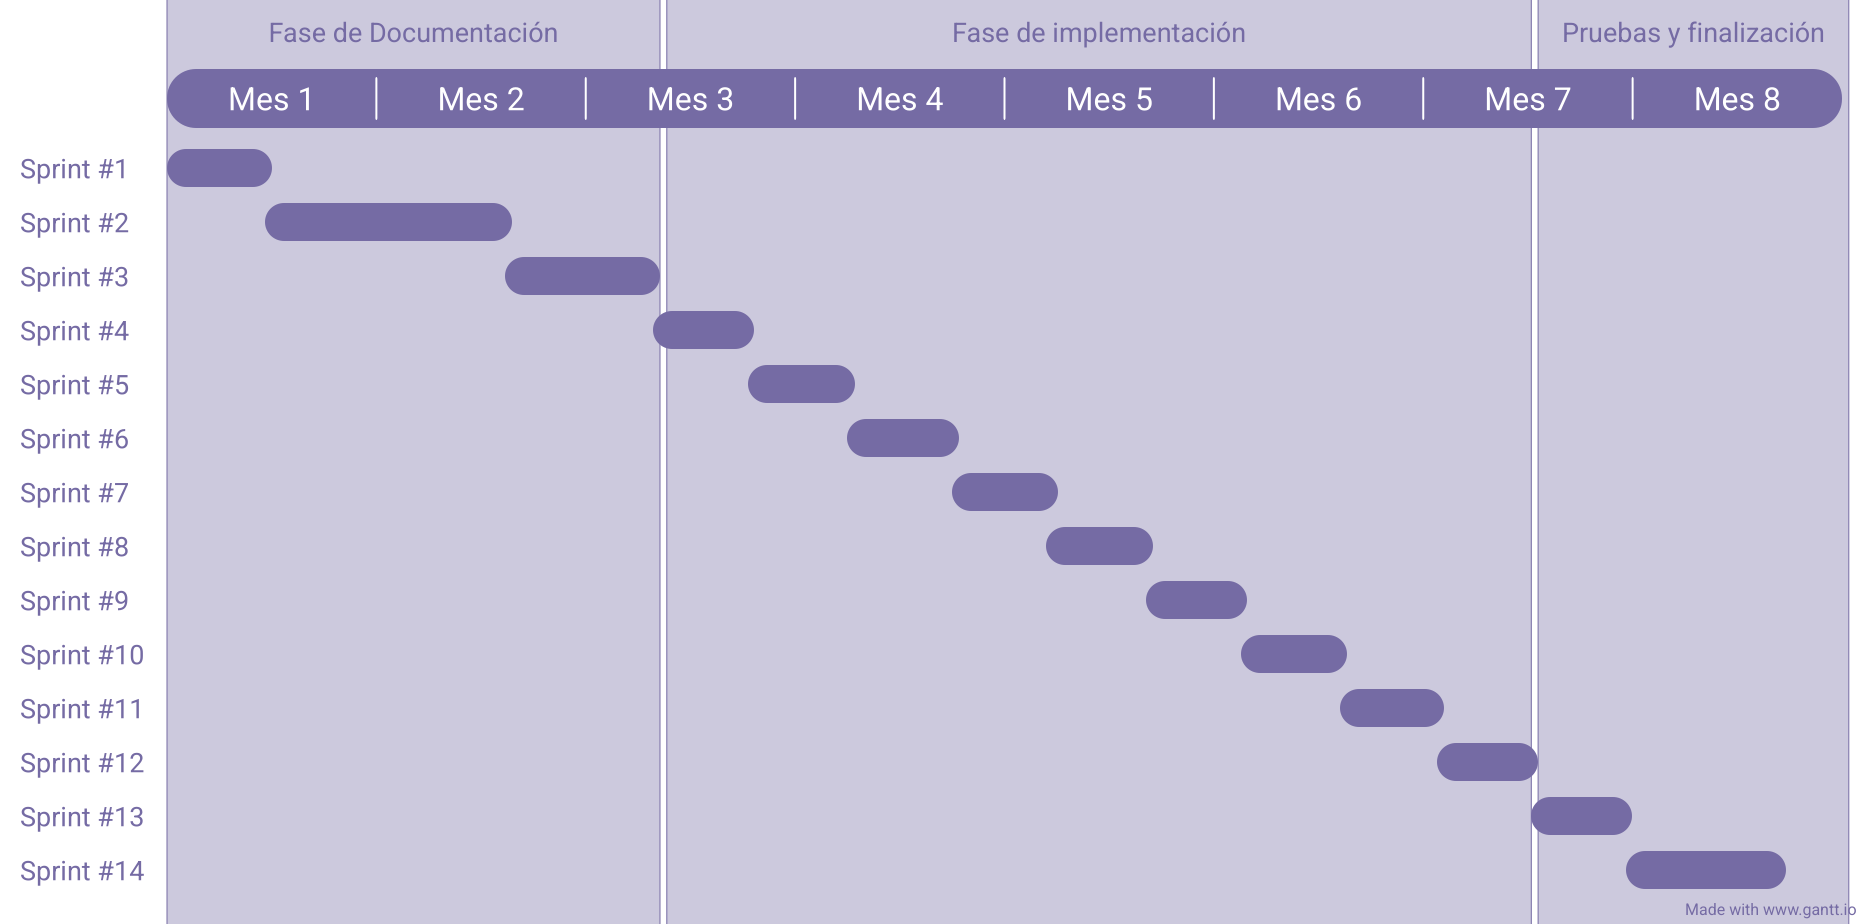
\includegraphics[width=1.25\textwidth]{imagenes/c4/gantt.png}}
    \caption{Diagrama de Gantt de la planificación del proyecto, divivido por Sprints.}
    \label{fig:diagrama_gantt}
    
    
\end{figure}